\documentclass[english]{thesis}
\usepackage[cpp]{mypackage}
\usepackage{hyperref}

\title{Homework 4}
\school{School of Data and Computer Science}
\author{Hongzheng Chen}
\stunum{17341015}
\headercontext{Parallel and Distributed Computing}

\begin{document}

\maketitle

\section{Problem 1}
Consider a sparse matrix stored in the \emph{compressed row format} (you may find a description of this format on the web or any suitable text on sparse linear algebra). Write an OpenMP program for computing the product of this matrix with a vector. Download sample matrics from the Matrix Market (\url{http://math.nist.gov/MatrixMarket}) and test the performance of your implementation as a function of matrix size and number of threads.

\bigskip

\textit{Answer.}
Since the matrix files downloaded from the Matrix Market are not in compressed row format, we have to transform the format first.
One matrix is stored using three arrays including \verb'row_offset', \verb'col_index', and \verb'val'.
When we obtain the three arrays, we can do the multiplication as the pseduocode shown below.
\begin{lstlisting}
for (int i = 0; i < numRows; ++i) {
	int offset = (i == numRows-1 ? numNonZeros : row_offset[i+1]);
	for (int j = row_offset[i]; j < offset; ++j)
		res[i] += vec[col_index[j]] * val[j];
}
\end{lstlisting}

The \verb'vec' is a predefined vector
\[\vv=\bmat{1 & 2 & \cdots & n}^\T\]
used for matrix-vector multiplication.

The code shown above is a sequential program for baseline comparison.
To obtain the OpenMP parallel program, we can directly add \verb'#pragma omp parallel for' before the outer for loop, since no dependency between two loops.

The experiment leverage ten datasets varying sizes collected from the Matrix Market, shown in Table~\ref{tab:benchmark}.
\begin{table}[H]
\caption{Benchmarks for experiments}
\label{tab:benchmark}
\centering
\begin{tabular}{|c|c|c|c|}\hline
\textbf{Benchmark} & \textbf{\# of rows} & \textbf{\# of cols} & \textbf{\# of non-zeros}\\\hline
\href{https://math.nist.gov/MatrixMarket/data/Harwell-Boeing/grenoble/gre__115.html}{gre} & 115 & 115 & 421\\\hline
\href{https://math.nist.gov/MatrixMarket/data/Harwell-Boeing/saylor/saylr1.html}{saylr} & 238 & 238 & 1128 \\\hline
\href{http://math.nist.gov/MatrixMarket/data/Harwell-Boeing/psadmit/1138_bus.html}{bus} & 1138 & 1138 & 2596\\\hline
\href{https://math.nist.gov/MatrixMarket/data/Harwell-Boeing/lanpro/nos3.html}{nos} & 960 & 960 & 8402\\\hline
\href{https://math.nist.gov/MatrixMarket/data/Harwell-Boeing/oilgen/orsreg_1.html}{orsreg} & 2205 & 2205 & 14133\\\hline
\href{https://math.nist.gov/MatrixMarket/data/Harwell-Boeing/sherman/sherman2.html}{sherman} & 1080 & 1080 & 23094\\\hline
\href{https://math.nist.gov/MatrixMarket/data/Harwell-Boeing/econaus/orani678.html}{orani} & 2529 & 2529 & 90158\\\hline
\href{https://math.nist.gov/MatrixMarket/data/Harwell-Boeing/bcsstruc2/bcsstk16.html}{bcsstk} & 4884 & 4884 & 147631\\\hline
\end{tabular}
\end{table}

And the machine used for the experiment equips with a Intel Core i7-7700HQ processor (8 cores) running at 2.80GHz and a 8GB memory.
The programs are compiled with gcc 7.3.0 and running on Ubuntu 18.04(LTS).

The experimental results\footnote{The figures of the experiments are created with Python Matplotlib, and the notebook \textit{plot.ipynb} is also in the attachment.} are shown in Fig~\ref{fig:scalability}.
Notice the scalability results of number of threads are for the biggest benchmark \verb'bcsstk'.
\begin{figure}[H]
\centering
\begin{tabular}{cc}
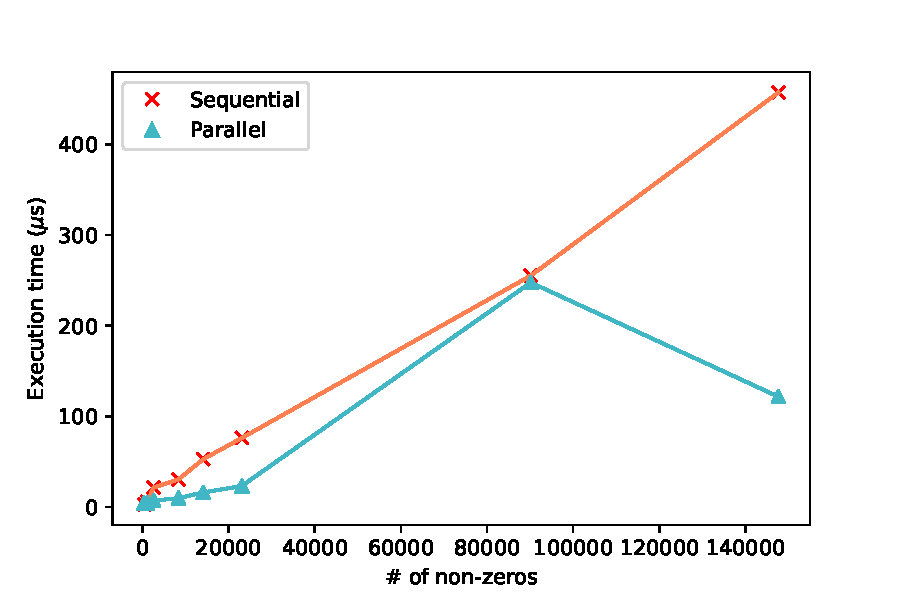
\includegraphics[width=0.5\linewidth]{fig/size.pdf}&
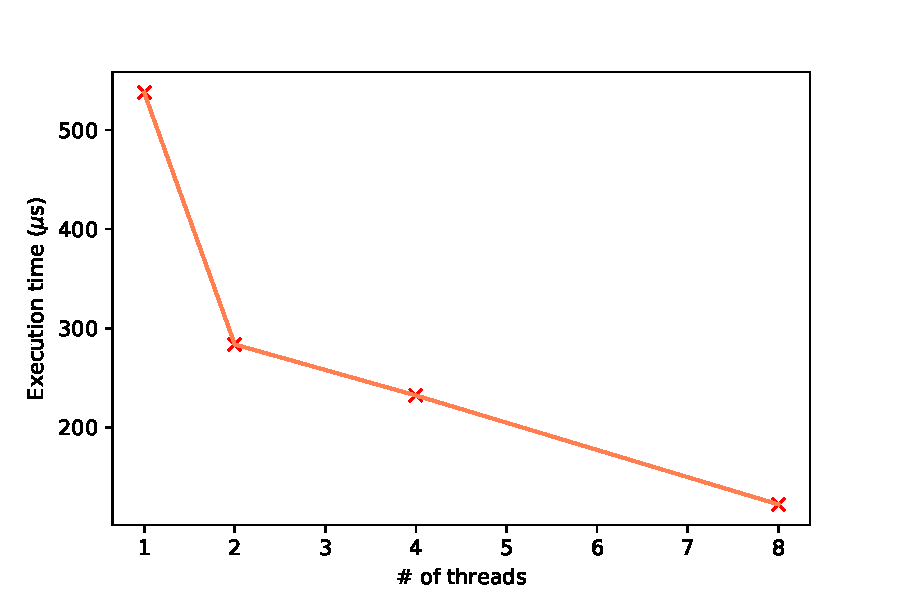
\includegraphics[width=0.5\linewidth]{fig/worker.pdf}
\end{tabular}
\caption{Scalability of matrix size and number of threads}
\label{fig:scalability}
\end{figure}

From Fig.~\ref{fig:scalability}, we can see that as the size of the matrix scales, the difference of the execution time between parallel and sequential programs becomes larger.
When more threads are considered, the speedup of the parallel program becomes larger, which is expected.

But we can also see that for the \verb'orani' benchmark, the running time of parallel program is similar to the sequential program, which results from the specific structure of the input matrix.
The matrix is asymmetric and unstructured (shown in Fig.~\ref{fig:orani}), thus using compressed row format to store and compute the matrix may not be a good choice.
\begin{figure}[H]
\centering
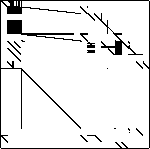
\includegraphics[width=0.3\linewidth]{fig/orani678.png}
\caption{Orani's matrix structure}
\label{fig:orani}
\end{figure}

I also add other features into my program for high productivity.
\begin{itemize}
	\item Use \verb'template' and \verb'typedef' for flexibility of different value types.
	\item Leverage \verb'<chrono>' header for high-accuracy timing.
	\item Write a \verb'Makefile' for auto compiling and experimenting.
\end{itemize}

The program \verb'matmul.cpp' can be found in the attachment.

\section{Problem 2}
Implement a producer-consumer framework in OpenMP using \verb'sections' to create a single producer task and a single consumer task. Ensure appropriate synchronization using locks. Test your program for a varying number of producers and consumers.

\bigskip

\textit{Answer.}
Similar to Project 1, we can emulate a queue by a fixed-size array, whose head and tail are connected as a ring.
Two operations \verb'push' and \verb'pop' are implemented for the queue.
In each operation. we leverage \verb'#pragma omp critical' to ensure the mutuality.

Each producer produces one number and push it into the queue.
The consumers pop the numbers from the queue and add them together.

The producers and consumers are encapsulated in \verb'omp section'.
All the sections are put in a large block \verb'omp parallel sections', which enables the sections to run in parallel.

The experimental results are shown in Table~\ref{tab:results}.
Due to time limitation, only several experiments are conducted here.

\begin{table}[H]
\centering
\caption{Running time of the producer-consumer framework}
\label{tab:results}
\begin{tabular}{|c|c|c|}\hline
\textbf{\# of producers} & \textbf{\# of consumers} & \textbf{Running time (ns)}\\\hline
2 & 2 & 2499500 \\\hline
2 & 6 & 3709500 \\\hline
4 & 4 & 2148600 \\\hline
6 & 2 & 1785100 \\\hline
8 & 8 & 2210600 \\\hline
\end{tabular}
\end{table}

From Table~\ref{tab:results}, we can see that more consumers lead to slower running time, which may result from the heavy conflicts of popping.
Once the number is produced, it may immediately be consumed by the consumers.
From these limited cases, we can also conclude that the more producers may be better for the performance.
Since no larger cases are tested, the conclusion may be different when the input size scales.

The program \verb'prod-cons.cpp' can be found in the attachment.
Notice at this time, the number of producers and consumers cannot be set automatically.
The default setting is two producers with two consumers.

\end{document}